\documentclass{article}
\usepackage{Preamble}


\title{Assignment 2: Linked Lists and Arrays \\[5pt] Part 1: Linked List Iterator \\[8pt] CS3305/W01 Data Structures}
\author{Casey Hampson}

\begin{document}
\maketitle



\section*{Program Output}
    Just to make extra sure it is understood: the output for $x=8$ and $y=5$ has nothing below it, which is what is intended. Also, I misread the instructions and didn't notice we could use Java's built-in LinkedList, so I just made my own. Good practice!

    \begin{figure}[htbp]
        \centering
        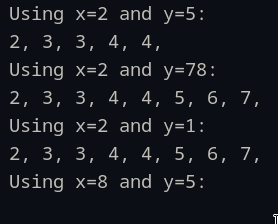
\includegraphics[scale=0.8]{./res/1.png}
        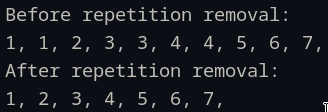
\includegraphics[scale=0.8]{./res/2.png}
    \end{figure}

\pagebreak
\section*{Source Code}
\inputminted{java}{./P1.java}


\end{document}
